When there is a delay in the time a sensor provides a measurement and the time it is made available for the measurement update, the estimation procedure needs to address this delay instead of naively incorporating the measurement into the corection step.
Similarly if a measurements is corrupted by an uncertain bias, it needs to be mitigated in the estimation process.
This article describes an approach to address the delay and bias in the measurement for a discrete-time estimation model.

\begin{figure}
	%trim={Left Bottom Right Top}
	% \fbox%
	{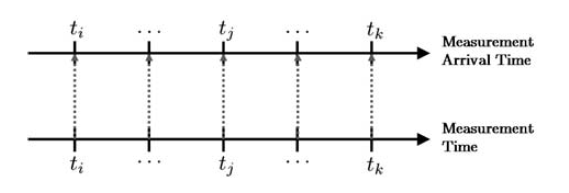
\includegraphics[width=1.0\columnwidth]{./img/undelayed_measurement.png}}
	\caption{Sequence of measurements unaffected by delay}
	\label{fig:undelayed_measurement}
\end{figure} 

\begin{figure}
	%trim={Left Bottom Right Top}
	% \fbox%
	{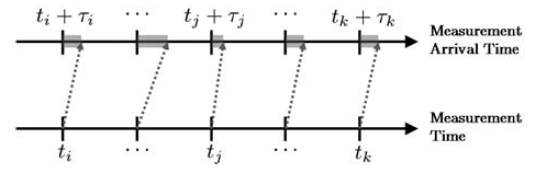
\includegraphics[width=1.0\columnwidth]{./img/delayed_measurement.png}}
	\caption{Sequence of measurements affected by delay}
	\label{fig:delayed_measurement}
\end{figure} 

\begin{figure}
	%trim={Left Bottom Right Top}
	% \fbox%
	{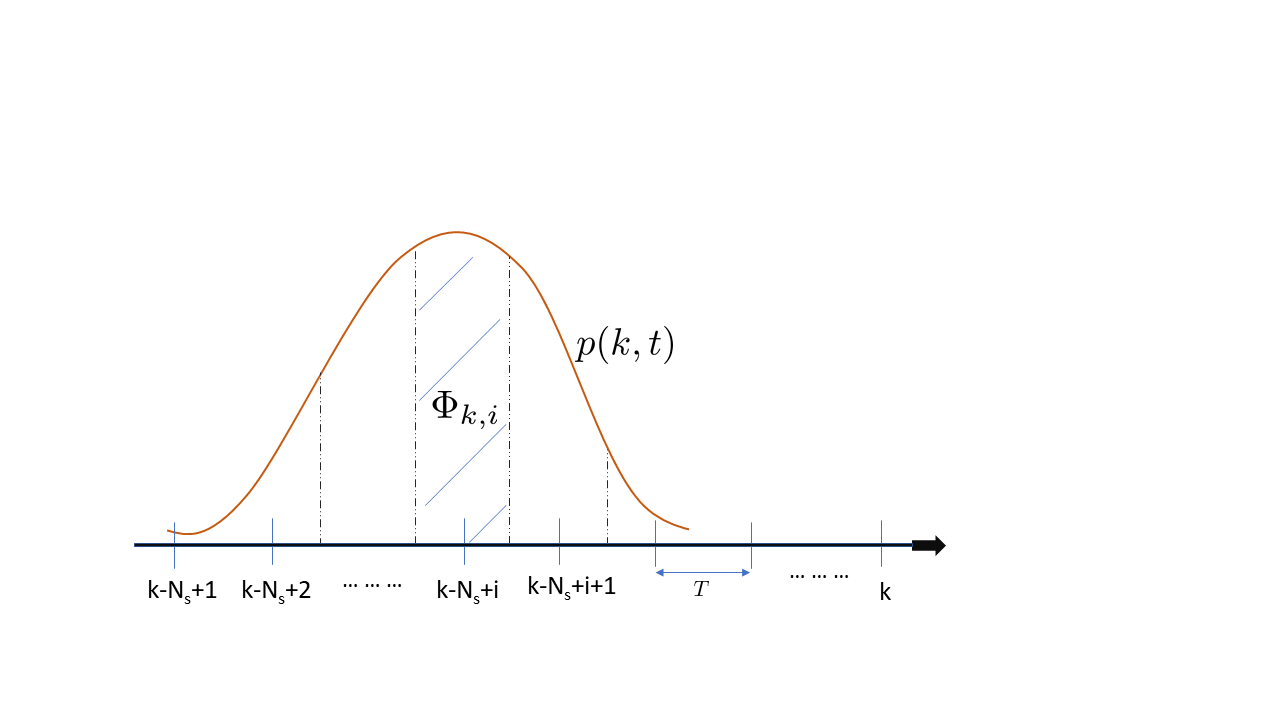
\includegraphics[width=1.0\columnwidth]{./img/delay_uncertainty.png}}
	\caption{Lag uncertianty for delayed measurement}
	\label{fig:delay_uncertainty}
\end{figure} 
 